\section{Algorytm rozpoznawania znaków}
Segmentacja obrazu prowadzi do wyodrębnienia z obrazu żądanych obiektów. Zwykle jest ona pierwszym etapem analizy całego obrazu. Odnalezione obiekty bardzo często poddawane są analizie w celu identyfikacji lub podjęcia decyzji.
\paragraph{}
W przypadku problemu rozpoznawania znaków, zadaniem algorytmu segmentacji jest określenie lokalizacji każdego znaku oraz binaryzacja fragmentów obrazu zawierającego tekst. Kolejnym krokiem jest dostarczenie serii wykadrowanych obrazów binarnych zawierających pojedyncze znaki do algorytmu rozpoznawania znaków. Zadaniem algorytmu rozpoznawania znaków jest określenie, jaki znak tekstu znajduje się na zadanym obrazie.
\paragraph{}
Poniżej zostanie opisanych kilka algorytmów rozpoznawania znaków.
\subsection{Rozpoznawanie na podstawie cech}
Cechy umożliwiają dopasowanie obiektu do danego wzorca, określając ich stopień podobieństwa. Cechami obiektu mogą być kształt czy kolor. Poniżej przedstawiono cechy, które mogą zostać użyte w celu identyfikacji znaku.
\subsubsection{Cechy geometryczne}
\subsubsection{Momenty geometryczne}
\subsubsection{Rzut jasności obiektu}
Metoda rzutu jasności obiektu została opisana w podrozdziale~\ref{ssection:rzut_jasnosci}. W pierwszej kolejności należy przeskalować obraz do rozmiarów obrazu wzorcowego, a następnie wykonać algorytm rzutu jasności zarówno w pionie, jak i w poziomie. Otrzymane rzuty zostają następnie poddane analizie podobieństwa z rzutami wykonanymi dla znaków wzorcowych. Analiza podobieństwa polega na porównaniu kształtu otrzymanych rzutów jasności. \\
Na rysunku~\ref{fig:rzut_jasnosci_ocr} przedstawione zostały wzorce kilku znaków, oraz przykładowy obraz wejściowy.

\begin{figure}
  \centering
  \begin{subfigure}[b]{0.42\textwidth}
    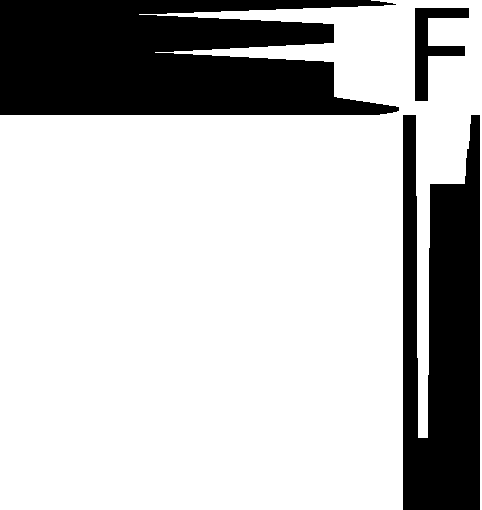
\includegraphics[width=\textwidth]{img/rzut-wzorzec-F}
    \caption{Wzorzec dla litery F}
    \label{fig:rzut_wzorzec_F}
  \end{subfigure}
  ~
  \begin{subfigure}[b]{0.42\textwidth}
    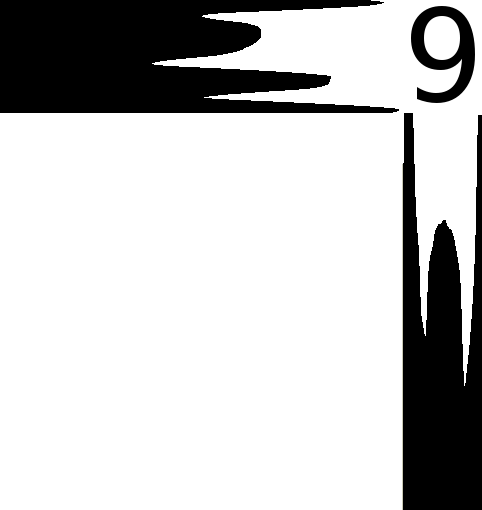
\includegraphics[width=\textwidth]{img/rzut-wzorzec-9}
    \caption{Wzorzec dla cyfry 9}
    \label{fig:rzut_wzorzec_9}
  \end{subfigure}
  \begin{subfigure}[b]{0.44\textwidth}
    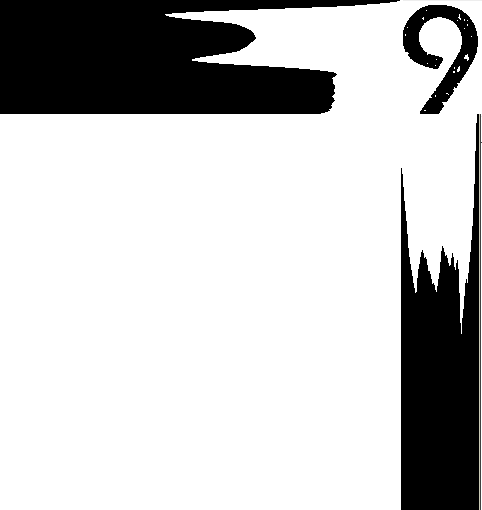
\includegraphics[width=\textwidth]{img/rzut-in-9}
    \caption{Obraz wejściowy, zawierający cyfrę 9}
    \label{fig:rzut_in_9}
  \end{subfigure}
  \caption{Porównanie rzutu jasności dla wybranych znaków}
    \label{fig:rzut_jasnosci_ocr}
\end{figure}
